\chapter{Caractérisation de l'échangeur ambiant}\label{chap:AHX}
Cette partie concerne la mesure de la chaleur extraite par l'échangeur ambiant $\dot Q_a$. Cet échangeur en cuivre conçu durant le projet \textsc{Tacot} et représenté sur la figure~\ref{fig:AHXschema} contient un circuit de canaux dans lequel circule de l'eau dont le débit peut être contrôlé \cite{ANR_thermo-acoustic_2019, ramadan_design_2021}. Son rôle est de maintenir l'extrémité chaude du régénérateur à température ambiante pour éviter l'échauffement globale du réfrigérateur. 

\begin{figure}[!ht]
    \centering
    \external{fig_AHXSchema}
    %\externalremake
    \begin{tikzpicture}
\draw (0,0) node {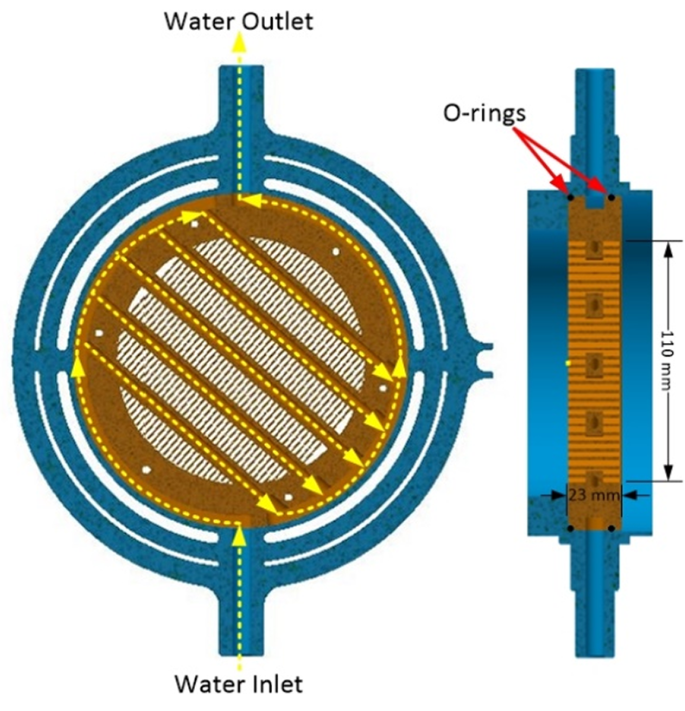
\includegraphics[width=.5\textwidth]{../fig/fig_AHXfromATE/AHXfromATE.png}};
    
\end{tikzpicture}
    \caption{Schéma de l'échangeur ambiant, issu de \cite{ramadan_design_2021}}
    \label{fig:AHXschema}
\end{figure}

Le but de cette étude est multiple : d'une part, l'alimentation en eau de l'échangeur se fait par un robinet puis est rejetée dans un évier, ce qui engendre un grand gaspillage. Son remplacement par un circuit fermé est prévu, mais il est nécessaire de connaître au préalable le débit nécessaire à un bon échange thermique. D'autre part, l'échange de chaleur dépend du débit d'eau $\dot q$ ainsi que de la différence de température de l'eau $\Delta T^w$ entre la sortie et l'entrée de l'échangeur. Cette dernière dépend également du débit, et le problème est donc de choisir le débit tel que la différence de température de l'eau soit la plus grande possible, tout en garantissant une extraction optimale de la chaleur par l'échangeur.

\section{Détermination de la chaleur pompée}
Tout d'abord, il est important de distinguer les flux de chaleur en jeu au niveau de l'échangeur ambiant. Le premier est celui qui transporte la chaleur de l'extrémité chaude du régénérateur à la partie solide l'échangeur ambiant, et le second, de cette partie solide de l'échangeur à l'eau qui y circule. Ils sont notés respectivement $Q_a'$ et $Q_a$, et c'est ce deuxième flux qu'il est possible d'estimer par la mesure de température d'eau.\smallskip

La quantité de chaleur extraite par l'eau à l'échangeur est définie par

\begin{equation}
    Q_a = m\ C_p\ \Delta T^w\quad,
    \label{eq:Qa_energie}
\end{equation}
où $m$ est la masse d'eau écoulée, $C_p$ la capacité calorifique de l'eau et $\Delta T^w$ la différence de température de l'eau entre l'entrée et la sortie de l'échangeur. La dérivée temporelle de cette équation donne la puissance thermique extraite par l'échangeur, qui s'écrit

\begin{equation}
    \dot Q_a = \dot m\ C_p\ \Delta T^w\quad,
    \label{eq:Qa_puissance}
\end{equation}

Pour prendre en compte l'écart intrinsèque aux capteurs de température, il est nécessaire de soustraire une différence $\Delta T_0^w$ qui correspond à l'écart de température de l'eau quand celle-ci circule dans l'échangeur, sans toutefois alimenter les sources acoustiques ni les charges thermiques\medskip

Les mesures de $\Delta T^w$ sont réalisées au moyen de sondes de platine PT100 pour les débits \qtylist{4.5;7;9.5}{\litre\per\minute} d'une eau à \qty{20}{\degreeCelsius}, et la chaleur extraite $\dot Q_a$ est déduite de ces mesures. Pour chaque débit, trois étapes sont réalisées : ouverture du robinet d'eau, puis démarrage des sources acoustiques, et enfin ajout d'une charge thermique $\dot Q_f$ du côté froid du régénérateur. Pour chacune de ces étapes, le régime transitoire ainsi que le régime établi sont acquis. Les résultats sont présentés figure~\ref{fig:AHXCalib} et représentent les quantités en régime établi. 

\begin{figure}[!ht]
    \centering
    \external{fig_AHXCalib}
%    \externalremake
    \begin{tikzpicture}
    \def\height{5cm};
    \def\width{.65\textwidth};
    \def\spx{1.2};
    \def\spy{.5cm};
    \def\legx{.5cm};
    \def\legy{.3cm};

    \begin{axis}[name=DTqdot,height=\height,width=\width, 
    x tick label style={
        /pgf/number format/1000 sep=},  
    %xlabel=$\dot q$ (\unit{\l\per\minute}),
    ylabel=$\Delta T^w$ (\unit{\degreeCelsius}),
    xmajorticks=false,
    ybar,enlarge x limits=.15,
    legend pos=outer north east]
    
    \addplot[solid,ultra thick,fill=MatlabBlue!25,draw=MatlabBlue] file {../fig/fig_AHXCalib/data/data_qdotDT0Water.txt};
    \addplot[solid,ultra thick,fill=MatlabOrange!25,draw=MatlabOrange,
    postaction={
        pattern=north east lines,pattern color=MatlabOrange
    }] file {../fig/fig_AHXCalib/data/data_qdotDT1WaterAcou.txt};
    \addplot[solid,ultra thick,fill=MatlabOrange!25,draw=MatlabOrange] file {../fig/fig_AHXCalib/data/data_qdotDT10Acou.txt};
    \addplot[solid,ultra thick,fill=MatlabYellow!25,draw=MatlabYellow,
     postaction={
        pattern=north east lines,pattern color=MatlabYellow
    }] file {../fig/fig_AHXCalib/data/data_qdotDT2WaterAcouQc.txt};
    \addplot[solid,ultra thick,fill=MatlabYellow!25,draw=MatlabYellow] file {../fig/fig_AHXCalib/data/data_qdotDT20AcouQc.txt};
    \legend{$\Delta T_0^w$ \\ $\Delta T_1^w$ \\ $\Delta T_1^w-\Delta T_0^w$ \\ $\Delta T_2^w$ \\ $\Delta T_2^w-\Delta T_0^w$ \\};
\end{axis}

\begin{axis}[name=Qdotqdot,height=\height,width=\width, 
    x tick label style={
        /pgf/number format/1000 sep=},  
    xlabel=$\dot q$ (\unit{\l\per\minute}),
    ylabel=$\dot Q_a$ (\unit{\watt}),
    xtick={4.5,7,9.5},
    ybar,enlarge x limits=.15,
    at={($(DTqdot.south)+(0,-\spy)$)},anchor=north,
    legend pos=outer north east]
    
    \addplot[solid,ultra thick,fill=MatlabOrange!25,draw=MatlabOrange] file{../fig/fig_AHXCalib/data/data_qdotQa1dotNoHeat.txt};
    \addplot[solid,ultra thick,fill=MatlabYellow!25,draw=MatlabYellow] file{../fig/fig_AHXCalib/data/data_qdotQa2dotHeat.txt};
    \legend{$\dot Q_f=0$ \\ $\dot Q_f \neq 0$ \\};
    \end{axis}
    
    \draw ($(DTqdot.north west)+(\legx,-\legy)$) node[]{\bf(a)};
    \draw ($(Qdotqdot.north west)+(\legx,-\legy)$) node[]{\textbf{(b)}};
\end{tikzpicture}
    \caption[Calibration de l'échangeur de chaleur ambiant.]{Calibration de l'échangeur de chaleur ambiant. \textbf{(a)} différence de température pour l'eau seule ($\Delta T_0^w$), après ajout des sources acoustiques en marche ($\Delta T_1^w$), puis après ajout d'une charge thermique $\dot Q_f$ ($\Delta T_2^w$). \textbf{(b)} puissance thermique $\dot Q_a$ extraite par l'eau en l'absence puis en présence d'une charge thermique $\dot Q_f$ côté froid.}
    \label{fig:AHXCalib}
\end{figure}




\section{Incertitudes de mesures}


\subsection{Température}
\echaf{blablabla}

\subsection{Débit d'eau}

La mesure du débit d'eau circulant dans l'échangeur ambiant est également source d'incertitude. En effet, le débitmètre à turbine utilisé \echaf{Marque, modèle} s'écarte de la valeur vraie du débit quand celui-ci est faible. Pour estimer l'écart à la réalité, la mesure par le débitmètre à turbine est comparé à celle par un débimètre à ultrason \echaf{vraiment le meilleur ? pourquoi ne pas utiliser l'ultrason pour toutes les manips ? pour la "valeur vraie", pourquoi pas un volume d'eau connu et un chrono ?}

\begin{figure}[!ht]
    \centering
    \external{fig_IncertitudeDebitEau}
%    \externalremake
    \begin{tikzpicture}
    \def\height{.9*\textwidth};
    \def\width{\height};
    \def\spx{.5cm};
    \def\spy{.5cm};
    \def\legx{.5cm};
    \def\legy{\legx};
    \def\prop{.45};
    
    \begin{axis}[name=TurbineUltrason,width={\width},height={\height},
    xlabel={$\dot q_{\textsf{us}}$ [\unit{\liter\per\minute}]},
    ylabel={$\dot q_{\textsf{tb}}$ [\unit{\liter\per\minute}]},
    xmin=0,xmax=10,ymin=0,ymax=10,
    domain=0:9.5,
    legend style = {at={(.97,.03)},anchor = south east}
    ]
        \addplot[solid,ultra thick,draw=MatlabBlue] file {../fig/fig_IncertitudeDebitEau/data/data_calibTurbineVSUltrason.txt} ;\addlegendentry{Exp.}
        \addplot[dashed,ultra thick,draw=MatlabBlue] {1.002*x - .3847}; \addlegendentry{Approx. linéaire,}
        \addlegendimage{empty legend}
        \addlegendentry{$\dot q_{\sf tb}=\dot q_{\sf us}-0.3847$}
        
%        \legend{Exp. \\ \begin{tabular}{l}Approx. linéaire\\$\dot q_{\sf tb}=\dot q_{\sf us}-0.3847$\end{tabular} \\};
    \end{axis}
    
    \begin{axis}[name=EcartRelat,width={\prop*\width},height={\prop*\height},
    xlabel={$\dot q$ [\unit{\liter\per\minute}]},
    ylabel={\'Ecart relatif $\epsilon$ [\unit{\percent}]},
    xmin=0,xmax=10,ymin=0,ymax=100,
    at={($(TurbineUltrason.north)+(\spx,-\spy)$)},anchor= north east
    ]
        \addplot[solid,ultra thick,draw=MatlabOrange] file {../fig/fig_IncertitudeDebitEau/data/data_RelativeDiff.txt};
    \end{axis}
    
    \draw ($(TurbineUltrason.north east)+(-\legx,-\legy)$) node[]{\bf (a)};
    \draw ($(EcartRelat.north east)+(-\legx,-\legy)$) node[]{\bf (b)};
    
\end{tikzpicture}
    \caption[Incertitudes de mesure du débit d'eau dans l'échangeur ambiant]{Incertitudes de mesure du débit d'eau dans l'échangeur ambiant. \textbf{(a)} débit mesuré par le débitmètre à turbine $\dot q_{\sf tb}$ en fonction de celui mesuré par le débitmètre à ultrason $\dot q_{\sf us}$. \textbf{(b)} écart relatif $\epsilon=\frac{|\dot q_{\sf us}-\dot q_{\sf tb}|}{\dot q_{\sf us}}$ entre les deux mesures obtenues.}
    \label{fig:IncertitudeDebitEau}
\end{figure}%

\echaf{Texte après le float}